\section{印度佛教史}

\subsection{种性制度}
\begin{itemize}
  \item 婆羅門:祭司
  \item 剎帝利:武士
  \item 吠舍: 农工商业
  \item 首陀羅: 奴隶
\end{itemize}

\subsection{六派哲學}
產生於史詩時期之末,與佛教初期階段相近的婆羅門教哲學\footnote{木村泰賢$\cdot$《原始佛教思想論》}。
\begin{itemize}
  \item 尼夜耶派(The Nyāya School)。
  \item 僧佉耶派(The Sāṃkhya School)即數論派。
  \item 毘舍迦派(The Vaiśeṣika School)即勝論派。
  \item 瑜伽派(The Yoga School)。
  \item 弭曼差派(The Mīmāṃsā School)。
  \item 吠檀多派(The Vedānta School)。
\end{itemize}

\subsection{奧義書}
\begin{itemize}
  \item 業說,在《古奧義書》本為不公開的密教,到佛世則成為各教派所公認的思想
  \item 輪迴說,在梵書時代已萌芽,完成而為一般所承認,則自奧義書時代始
  \item 解脫說,乃為《奧義書》的最終目的
\end{itemize}

\subsection{六師外道}
記載常見於声闻經律\footnote{《長阿含經》第二十七經《沙門果經》}
\begin{itemize}
  \item 不蘭迦葉(Pūraṇa-Kāssapa):為倫理的懷疑者,否定善惡之業有其相應之根,故倡無作用論。
  \item 末伽梨瞿舍利(Makkhali Gosāla):此為邪命外道之祖,倡無因而有論。乃是耆那教的一派,在佛世極有勢力,除了耆那教,他是其餘五師中最盛大者。
  \item 阿耆多翅舍欽婆羅(Ajita Keśakambala):否定靈魂之說,倡唯物論,以快樂為人生之目的,排斥一切嚴肅的倫理觀念,此亦即是順世外道。
  \item 婆浮陀伽旃那(Pakudha Kaccāyana):主張心物永不消滅,倡世間常存論。
  \item 散若夷毘羅梨沸(Sañjaya Belaṭṭhiputta):為詭辯派或捕鰻論者,舍利弗(Śāriputra)及目犍連(Mahāmaudgalyāyana),即是此派出身而皈信佛教的。
  \item 尼乾陀若提子(Nigaṇṭha-Nātaputta):這就是耆那教之始祖摩訶毘盧(Mahā-vira),他出世稍早於釋尊,也是王子出身。此派以命(Jīva)及非命之(Ājīva)之二元論而說明一切,故也是否定有上帝造物觀念的無神論者。其實踐方面,則以極端的苦行及嚴守不殺生為特色。
\end{itemize}

\subsection{六十二見}
兩說及十類\footnote{《長阿含經》卷一四第二十一經《梵動經》}
\begin{itemize}
  \item 說過去世,或稱本劫本見者,五類十八見:
    \begin{itemize}
      \item 世間常住論,即是常見論,四種。
      \item 世間半常半無常論,四種。
      \item 世間有邊無邊論,四種。
      \item 異問異答論,即是詭辯派、捕鰻論、不死矯亂論,四種。
      \item 無因而有論,即是無因論,二種。
    \end{itemize}
  \item 說未來世,或稱末劫末見者,五類四十四見:
    \begin{itemize}
      \item 世間有想論,十六種。
      \item 世間無想論,八種。
      \item 世間非有想非無想論,八種。
      \item 眾生斷滅無餘論,即是斷見論,七種。
      \item 現法涅槃論,即無論在何種狀態,處於現世的即為最高的境界,五種。
    \end{itemize}
\end{itemize}

\subsection{家谱}
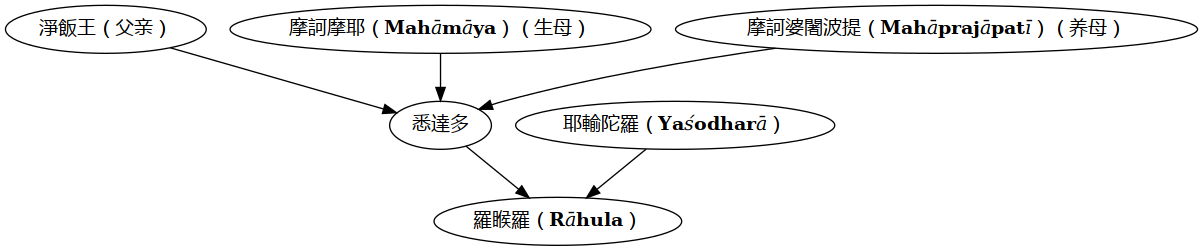
\includegraphics[width=\textwidth]{释家/images/释尊家谱.png}

\subsection{修道}
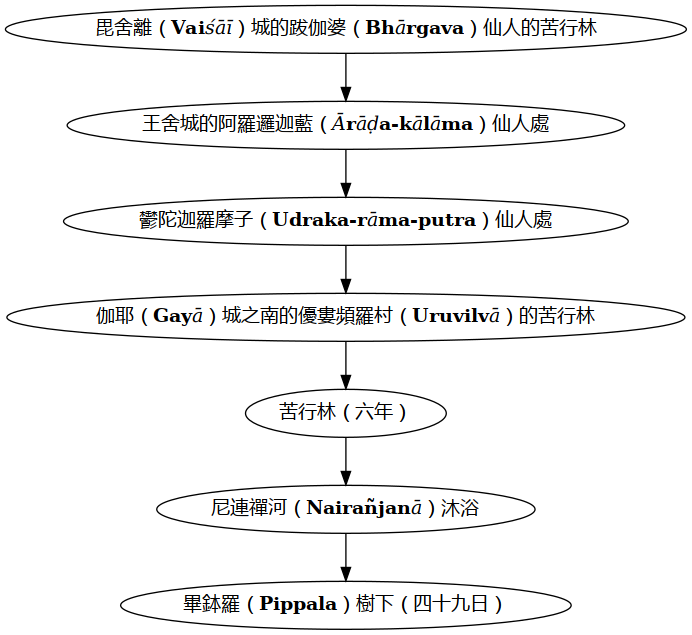
\includegraphics[width=\textwidth]{释家/images/释尊修行地图.png}

\subsection{四七日}
\begin{enumerate}
  \item 在菩提(Bodhivṛkṣa)樹下。就是那棵畢鉢羅樹之下,因佛在此樹下成道,而被稱為菩提樹
  \item 在阿踰波羅(Ajapāla)樹下。此期有魔王波旬(Māra-pāpīmān)來請佛入滅而未果。
  \item 在目真鄰陀(Mucilinda)樹下,遇暴風雨,目真鄰陀龍見之而即以己身護佛。此龍即受皈依,乃為傍生中的第一弟子。
  \item 在羅闍耶恆那(Rājāvatana)樹下。有二商主,一名提謂,一名婆梨迦,道經佛處,以麨蜜供佛,並皈依佛、法而去。此二人乃為最早的優婆塞(Upāsaka 親近而奉事三寶的淨信男)
\end{enumerate}

\subsection{轉法輪}
\begin{enumerate}
  \item 婆羅奈斯(Vārāṇiasī)城的鹿野苑度五比丘,接著又度了耶舍(Yaśa)及其親友數十人
    \footnote{ 阿若憍陳如(Ājñāta-Kauṇḍinỵa)、跋提(Bhadrika)、婆波(Vāṣpa)、摩訶男(Mahānāma)阿說示(Aśvajit)}
    \footnote{自此即有了教主、教法、教團的(佛、法、僧)三寶具足}
    \footnote{滿慈子、大迦旃延、婆毘耶等,亦捨外道法而進入佛法。}
    。
  \item 在鹿野苑度過第一個雨季的安居生活,釋尊便囑咐弟子們各各遊化人間,弘揚佛陀的教義
    \footnote{乃至要弟子們不應兩個人同走一條路};
    佛陀自己也單獨去到優婁頻羅聚落
    \footnote{化度了事火外道優婁頻羅迦葉(Uruvilvā-kāśyapa)和他的兩個弟弟那提迦葉(Nadī-kāśyapa)、伽耶迦葉(Gayā-kāśyapa),以及他們三人的弟子共一千人。}
    。
  \item 釋尊為了履行成道之後去度頻婆沙羅王的諾言,便率領迦葉三兄弟及其弟子們到了王舍城,國王
    \footnote{見到聞名於當時的迦葉三兄弟,均已成了佛的弟子,信心益加懇切,聞法之下,即得法眼淨(見道)。}
    親率臣民迎於郊外;迦蘭陀(Kalanda)長者將他在王舍城外的竹園施佛,王即為佛陀在此園中建造精舍
    \footnote{這是第一所大規模的佛教道場}
    。
  \item 佛陀成道第四年,六師外道之一的詭辯派的名匠舍利弗於言下
    \footnote{「諸法因緣生,諸法因緣滅」,「諸行無常,是生滅法,生滅滅已,寂滅為樂」}
    得法眼淨,和同門知友大目犍連各率弟子共二百五十人,詣佛出家,證阿羅漢果;
    又有摩訶迦葉(Mahā-kāśyapa)\footnote{「若不值佛,亦當獨覺。」}迴心進入釋尊的法海
    \footnote{佛經中常見的「千二百五十人俱,皆是大阿羅漢」的教團,到此便已形成。}
    。
  \item 佛陀成道第五年,即受到憍薩羅國(Kośala)首都舍衛城(Śrāvastī)的禮請,那就是須達(Sudatta 又作須達多)長者以重價購了一座祇樹給孤獨園奉施佛陀,作為弘法的中心。
  \item 同年,釋尊也應父王之召,回到祖國迦毘羅衛省親,父王預建精舍於尼拘律園,以接待釋尊。
    釋尊為父王說法,淨飯王即在聽法之際得法眼淨,宮人也多受了戒法,並度了異母弟(摩訶婆闍波提所生的)難陀,以及佛陀的親子羅睺羅出家。
    這次回國一共住了七天,便辭別父王返至王舍城,但卻在釋尊的座下,因此而增加了許多由釋迦王族來出家的弟子們
    \footnote{其中著名的,就有阿那律(Aniruddha)、阿難(Ānanda)、金毘羅(Kumbhīra)、提婆達多(Devadatta)等的追踪而至;為王子們理髮的賤民優波離(Upāli),亦於此時趕來出家,並且得到佛陀的特別優遇,讓他出家在諸王子之先,一則為表佛法的平等,一則為抑制諸王子驕傲的習氣。}
    \footnote{後世傳稱的佛陀的十大弟子,除了須菩提(Subhūti)似乎出家較遲而外,到此為止,其他的九位,均已出現了。}
    。
  \item 自釋尊成道第六年後,即沒有詳細的年月及活動的地點可考\footnote{《僧伽羅剎所集經》列記佛陀歷年雨安居的所在}。
  \item 經過四十五年的化度,召集全體比丘們在毘舍離的竹林精舍會齊,做最後一次重要的教誨;最後到了拘尸那羅城外的娑羅(Śāla)樹林入滅
    \footnote{一位叫作須跋陀羅(Subhadra)的外道成為佛陀最後得度的弟子。}
    \footnote{《長阿含經》卷四第二經《遊行經》:「是故比丘,無為放逸,我以不放逸故,自致正覺。無量眾善,亦由不放逸得。一切萬物,無常存者。此是如來末後所說。」}
    \footnote{《佛遺教經》:汝等比丘,常當一心,勤求出道,一切世間動不動法,皆是敗壞不安之相……是我最後之所教誨。」}
    。
\end{enumerate}


\subsection{原始佛教}
\begin{quote}
  是指佛陀在世時的言行,以及經過佛陀親自印可了的弟子們的言行。這唯有從《阿含經》及律部中去找,而《阿含經》比律部更可信賴。
\end{quote}
\begin{quote}
  開示的內容不外四聖諦、十二因緣、八正道等。
\end{quote}
\begin{quote}
  先以人天法,使你法天法人,使你成為一個可敬的人,當你善根增長皈依三寶,受持五戒之後,再用解脫法門開示你。人天善法是一般人共同信守的,解脫法門則是佛陀獨自證悟經驗的。
\end{quote}
\begin{quote}
  佛弟子們應當重視佛陀應化的重心,是著重於人生的修為而至無明的解脫,不必以為佛陀已將一切的問題給我們做了解答。佛陀的任務在此而不在彼,不要捨本逐末,否則自己鑽進了死角,還要埋怨,那是咎由自取。
\end{quote}
\begin{quote}
  佛陀既以人生的無明之解脫為著眼,人生的主宰則在於「心」,心不能自主,因為心的特性是念念相續地活動變異,故為無常,無常即無主體可覓,故為無我。
\end{quote}

\subsection{经典结集}
\subsubsection{第一次}
  迦葉尊者\footnote{錫蘭《大史》第三章}自佛涅槃地趕至王舍城,由於阿闍世王的外護,即在毘婆羅(Vebhāra)山側的七葉窟(Sapta-parṇa-guhā)前,建築精舍,集合五百位大比丘,作為佛滅後第一次的雨安居處。在此安居期間,自第二個月開始一連七個月(北傳謂三個月),從事結集的工作。首由優波離誦出律藏,次由阿難誦出法藏。此即稱為「五百集法毘尼」,或稱「王舍城結集」,又名「第一結集」
  \footnote{僅是迦葉一派的人,是少數人的結集,是代表上座比丘之中苦行派的一個大會。}
  ;當王舍城的結集終了,在南傳《善見律》、北傳《四分律》、《五分律》,都說有一位富蘭那長老\footnote{釋尊第七位比丘,是耶舍的四友之一, 而不是說法第一的富樓那。},率領了五百比丘從南方來到王舍城,亦說是南山(Dakkhiṇa-giri)來,重新與大迦葉論法及律。
  第一結集的戒律內容,便是代表上座精神的標記,並為上座們鞏固了領導的地位。
\subsubsection{第二次}
薩婆伽羅、離婆多、三菩提、耶舍、修摩那、沙羅、富闍蘇彌羅、婆薩摩伽羅摩,加上一位受戒僅五歲而堪任教化並精識法律的敷坐具之人阿耆多(或阿夷頭),共九人。
九人的審查辯論,實際是代表了七百人的大會,故此稱為七百結集。
\paragraph{十事非法的問題}
此一大會,起因雖為乞錢,討論內容則共有十項,稱為跋耆比丘的十事非法,那便是:
\begin{itemize}
  \item 角鹽淨:即是聽貯食鹽於角器之中。
  \item 二指淨:即是當計日影的日晷,未過日中之後(橫列)二指的日影時,如未吃飽,仍可更食。
  \item 他聚落淨:即在一食之後,仍可到另一聚落復食。
  \item 住處淨:即是同一教區(界內)的比丘,可不必同在一處布薩。
  \item 隨意淨:即於眾議處決之時,雖不全部出席,但仍有效,只要求得他們於事後承諾即可。
  \item 所習淨:隨順先例。
  \item 生和合(不攢搖)淨:即是得飲未經攪拌去脂的牛乳。
  \item 飲闍樓㘈淨:闍樓㘈是未發酵或半發酵的椰子汁,得取而飲之。
  \item 無緣坐具淨:即是縫製坐具,可不用貼邊,並隨意大小。
  \item 金銀淨:即是聽受金銀。
\end{itemize}
毘舍離的跋耆比丘,以此十事可行,為合法(淨)\footnote{「吾滅度後,應集眾僧,捨微細戒。」};
上座耶舍,則以此為不合律制,為非法\footnote{「隨佛所說,當奉行之,佛不說者,此莫說也。」}。
第二次結集的目的,即在審查此十事的律制根據。其結果,據各律典的記載,上座代表們一致通過,認為十事非法。

\subsubsection{第三次}
上座系所出的三說:
\begin{itemize}
  \item 犢子系的傳說:佛滅百三十七年,波吒釐子城有魔,名眾賢,作羅漢形,與僧共諍十六年,遂有犢子比丘,集和合僧而息其諍,那時的護法者,為難陀王。故名第三結集。
  \item 分別說系的傳說:佛滅二百三十年頃,華氏城(Pāṭaliputta)有賊住比丘起諍,阿育王迎目犍連子帝須(Moggaliputta-Tissa),集千比丘而息諍,是為第三結集。
  \item 一切有系的傳說,佛滅四百年,迦膩色迦王因信說一切有部,集五百大德於迦濕彌羅,集三藏而裁正眾多的異說。
\end{itemize}

\subsubsection{第四次}

\subsubsection{六部律藏}
\begin{itemize}
  \item 南傳上座部\footnote{上座部應先於大眾部,可是南方的上座部,實是上座部中偏於大眾部的分別說系之一支,故仍較《摩訶僧祇律》為後出,其他四部也屬上座部的分部所出,上座根本部的律藏,今已無從求得了。}的Vinayapiṭaka,巴利文。
  \item 大眾部的《摩訶僧祇律》四十卷,東晉佛陀跋陀羅共法顯譯。
  \item 化地部的《五分律》三十卷,劉宋佛陀什共智勝譯。
  \item 法藏部的《四分律》六十卷,姚秦佛陀耶舍共竺佛念譯。
  \item 摩偷羅有部的《十誦律》六十一卷,姚秦鳩摩羅什譯。
  \item 迦濕彌羅有部的《根本說一切有部毘奈耶》五十卷,唐義淨譯。
\end{itemize}

\subsubsection{法}
法的遞演,經過三期而後大定:
\begin{enumerate}
  \item 集佛陀的言行為九部經(九分教)
  \item 演九部經為四《阿含經》
  \item 依四《阿含經》而立雜藏\footnote{由雜藏而出大乘藏、禁咒藏,那是大乘的範圍了}。
\end{enumerate}
\paragraph{九部經}
\begin{itemize}
  \item 修多羅(Sūtra):即是散文的說法,通稱為長行。
  \item 祇夜(Geya):以韻文重將所說散文的內容頌出,通常譯為應頌或重頌。
  \item 伽陀(Gāthā):說法時全以韻文宣出,譯作孤頌或諷誦。
  \item 尼陀那(Nidāna):記述佛及弟子的事蹟、始終、本末,因以事緣常為說法之助緣,故譯為因緣。
  \item 阿鉢陀那(Avadāna):以譬喻說法,或凡因事而興感,皆名譬喻。
  \item 闍多伽(Jātaka):佛陀自說過去世的因緣,兼及重要弟子們的宿行,故稱為本生。
  \item 伊帝目多伽(Itivṛttaka):敍述古佛的化跡,故稱本事。
  \item 阿浮達摩(Adbhuta-dharma):明佛及弟子種種不思議的神跡奇行者,故稱未曾有,新譯為阿毘達磨。
  \item 優波提舍(Upadeśa):對於甚深而簡要的法義,用問答方式來解說,故稱為論義,後世的論藏,即脫胎於此。
\end{itemize}
在這九部經中,以前三部為最古而最近於原形佛典,故與今之《雜\footnote{雜為相應之意,乃為原始結集的舊制。}阿含經》相當;
至於第四部因緣至第八部之未曾有,此五部為釋尊景行之類集,性質與前三部大不相同\footnote{實則九部經的後六部,即由前三部中分出,初次結集時,是否已有九部之名,乃為近世學者置疑。}。
\paragraph{十二部经}
上九部之外,加上優陀那(Udāna)(即鄔陀南)即無問自說、毘佛略(Vaipulya)即方廣、和伽羅(Vyākaraṇa)即授記。

\subsubsection{阿含}
阿含是梵語,新譯為阿笈摩(Āgama),義為法歸,有萬法歸趣於此而無遺漏的意思。用巴利語,則名為尼柯耶(Nikāya),其義為集或部。
\begin{itemize}
  \item 一切有部有雜、長、中、增一,共四《阿含經》,今存《雜阿含經》及《中阿含經》
  \item 化地部加雜藏,成五《阿含經》,今均不存
  \item 法藏部亦有五《阿含經》,今僅存《長阿含經》
  \item 大眾部也有五《阿含經》,今僅存《增一阿含經》
  \item 南傳有巴利語的五《尼柯耶》。
\end{itemize}
\paragraph{漢譯四《阿含經》vs 南傳的五《尼柯耶》}
\begin{itemize}
  \item 北傳《長阿含經》,二十二卷三十經;南傳《長部》(Dīghanikāya),分為三品三十四經。
  \item 北傳《中阿含經》,六十卷二二二經;南傳《中部》(Majjhimanikāya),分為十五品一五二經,其中有九十八經完全與北傳一致。
  \item 北傳《雜阿含經》,五十卷一三六二經;南傳《相應部》(Saṁyuttanikāya),分為五品二八八九經。
  \item 北傳《增一阿含經》,五十一卷千經以上,南傳《增支部》(Aṅguttaranikā-ya),分為一七二品二九一經,覺音以為其有九五五七經。
  \item 南傳《小部》(Khuddakanikya),),大小十五經,其中主要的有六種:
    \begin{enumerate}
      \item 法句(Dhammapada),相當漢譯的《法句經》及《法句譬喻經》。
      \item 自說經(Udāna),此即優陀那,漢譯中沒有。
      \item 本事(Itivuttaka)相當漢譯的《本事經》。
      \item 經集(Suttanipata),相當漢譯的《義足經》,即是古之義品、波羅延等。
      \item 長老、長老尼偈(Thera-theri-gatha),漢譯中無。
      \item 本生(Jātaka),相當漢譯的《生經》。
    \end{enumerate}
\end{itemize}
\paragraph{得名}
\begin{itemize}
  \item 《雜\footnote{《雜阿含經》是將佛世的法義,化繁為簡,做提綱挈領的摘要}阿含經》\footnote{西系上座之深入西北者,尊《雜阿含經》},即隨事義之相應者如修多羅、祇夜、伽陀等類別而編次之,例如處與處相應為一類,界與界相應又為一類,故南傳稱為《相應部》,其義相應而文則雜碎,故名《雜阿含經》,非如《開元釋教錄》解為「雜糅不可整理」之意。
  \item 《中阿含經》及《長阿含經》\footnote{西系之別為中系(分別說系)者,尊《長阿含經》},乃是以篇幅的長短得名,經文不長不短者名《中阿含經》,經文很長,則名《長阿含經》。
  \item 《增一阿含經》\footnote{東系的大眾部則尊《增一阿含經》},是以數字相次而集經,一而二,二而三,一一增加,乃至多法,故名增一。
\end{itemize}
